\documentclass{beamer}
\usepackage[utf8]{inputenc}
\usepackage{graphicx, epsfig}
\usepackage{amsmath,mathrsfs,amsfonts,amssymb}
%\usepackage{subfig}
\usepackage{floatflt}
\usepackage{epic,ecltree}
\usepackage{mathtext}
\usepackage{fancybox}
\usepackage{fancyhdr}
\usepackage{multirow}
\usepackage{enumerate}
\usepackage{epstopdf}
\usepackage{multicol}
\usepackage{algorithm}
\usepackage[noend]{algorithmic}
\usepackage{tikz}
\usepackage{blindtext}
\usetheme{default}%{Singapore}%{Warsaw}%{Warsaw}%{Darmstadt}
\usecolortheme{default}
\setbeamerfont{title}{size=\Huge}
\setbeamertemplate{footline}[page number]{}


\makeatletter
\newcommand\HUGE{\@setfontsize\Huge{35}{40}}
\makeatother    

\setbeamerfont{title}{size=\HUGE}
\beamertemplatenavigationsymbolsempty

% latin bold lower
\newcommand{\ba}{\mathbf{a}} 
\newcommand{\bc}{\mathbf{c}} 
\newcommand{\be}{\mathbf{e}} 
\newcommand{\bh}{\mathbf{h}} 
\newcommand{\bp}{\mathbf{p}} 
\newcommand{\bt}{\mathbf{t}} 
\newcommand{\bs}{\mathbf{s}} 
\newcommand{\bu}{\mathbf{u}} 
\newcommand{\bv}{\mathbf{v}} 
\newcommand{\bw}{\mathbf{w}} 
\newcommand{\bx}{\mathbf{x}} 
\newcommand{\by}{\mathbf{y}} 
\newcommand{\bz}{\mathbf{z}} 

% latin bold upper
\newcommand{\bA}{\mathbf{A}} 
\newcommand{\bB}{\mathbf{B}} 
\newcommand{\bC}{\mathbf{C}} 
\newcommand{\bI}{\mathbf{I}} 
\newcommand{\bL}{\mathbf{L}} 
\newcommand{\bM}{\mathbf{M}} 
\newcommand{\bQ}{\mathbf{Q}} 
\newcommand{\bT}{\mathbf{T}} 
\newcommand{\bU}{\mathbf{U}} 
\newcommand{\bV}{\mathbf{V}} 
\newcommand{\bW}{\mathbf{W}} 
\newcommand{\bX}{\mathbf{X}} 
\newcommand{\bY}{\mathbf{Y}} 
\newcommand{\bZ}{\mathbf{Z}} 

% latin cal upper
\newcommand{\cG}{\mathcal{G}} 
\newcommand{\cL}{\mathcal{L}} 
\newcommand{\cN}{\mathcal{N}} 
\newcommand{\cS}{\mathcal{S}} 
\newcommand{\cT}{\mathcal{T}} 
\newcommand{\cW}{\mathcal{W}} 
\newcommand{\cX}{\mathcal{X}} 
\newcommand{\cZ}{\mathcal{Z}} 

% latin bb upper
\newcommand{\bbE}{\mathbb{E}} 
\newcommand{\bbI}{\mathbb{I}} 
\newcommand{\bbP}{\mathbb{P}} 
\newcommand{\bbR}{\mathbb{R}} 

% greek bold lower
\newcommand{\bepsilon}{\boldsymbol{\epsilon}} 
\newcommand{\btheta}{\boldsymbol{\theta}} 
\newcommand{\blambda}{\boldsymbol{\lambda}} 
\newcommand{\bpi}{\boldsymbol{\pi}} 
\newcommand{\bmu}{\boldsymbol{\mu}} 
\newcommand{\bsigma}{\boldsymbol{\sigma}} 
\newcommand{\bphi}{\boldsymbol{\phi}} 

% greek bold upper
\newcommand{\bSigma}{\boldsymbol{\Sigma}} 

\DeclareMathOperator*{\argmin}{arg\,min}
\DeclareMathOperator*{\argmax}{arg\,max}

\newcommand{\createdgmtitle}[1]{\title[\hbox to 56mm{Deep Generative Models  \hfill\insertframenumber\,/\,\inserttotalframenumber}]
	{\vspace{1.5cm} \\ Deep Generative Models \\ {\Huge Lecture #1}}
	\author{Roman Isachenko}
	\institute{
	Moscow Institute of Physics and Technology
	} 
	\date{Autumn, 2021}
}

\newcommand\myfootnote[1]{%
  \tikz[remember picture,overlay]
  \draw (current page.south west) +(1in + \oddsidemargin,0.5em)
  node[anchor=south west,inner sep=0pt]{\parbox{\textwidth}{%
      \rlap{\rule{10em}{0.4pt}}\raggedright\scriptsize \textit{#1}}};}

\newcommand\myfootnotewithlink[2]{%
  \tikz[remember picture,overlay]
  \draw (current page.south west) +(1in + \oddsidemargin,0.5em)
  node[anchor=south west,inner sep=0pt]{\parbox{\textwidth}{%
      \rlap{\rule{10em}{0.4pt}}\raggedright\scriptsize\href{#1}{\textit{#2}}}};}
\createdgmtitle{6}
%--------------------------------------------------------------------------------
\begin{document}
%--------------------------------------------------------------------------------
\begin{frame}[noframenumbering,plain]
%\thispagestyle{empty}
\titlepage
\end{frame}
%=======
\begin{frame}{Recap of previous lecture}
	\vspace{-0.5cm}
	\begin{block}{Flow log-likelihood}
		\vspace{-0.3cm}
		\[
			\log p(\bx|\btheta) = \log p(f(\bx, \btheta)) + \log \left|\det \left( \frac{\partial f(\bx, \btheta)}{\partial \bx} \right) \right|
		\]
		\vspace{-0.5cm}
	\end{block}
	The main challenge is a determinant of the Jacobian.
	\begin{block}{Residual flows: planar/Sylvester}
		\vspace{-0.7cm}
		\[
			g(\bz, \btheta) = \bz + \mathbf{u} \, \sigma(\bw^T\bz + b); \quad 
			g(\bz, \btheta) = \bz + \bA \, \sigma(\bB\bz + \mathbf{b}).
		\]
		Matrix determinant lemma for calculating the Jacobian.
	\end{block}
	\begin{block}{Autoregressive flows}	
		\vspace{-0.4cm}
		\[
			x_i = \tau (z_i, c(\bz_{1:i-1})) \quad \Leftrightarrow \quad z_i = \tau^{-1} (x_i, c(\bz_{1:i-1}))
		\]
		Jacobian is triangular.
	\end{block}
	\myfootnote{\href{https://arxiv.org/abs/1505.05770}{Rezende D. J., Mohamed S. Variational Inference with Normalizing Flows, 2015}\\
	\href{https://arxiv.org/abs/1803.05649}{Berg R. et al. Sylvester normalizing flows for variational inference, 2018} \\
	\href{https://arxiv.org/abs/1705.07057}{Papamakarios G., Pavlakou T., Murray I. Masked Autoregressive Flow for Density Estimation, 2017}}
\end{frame}
%=======
\begin{frame}{Recap of previous lecture}
	\begin{block}{Gaussian autoregressive flow (MAF)}
		\vspace{-0.8cm}
		\begin{align*}
			\bx &= g(\bz, \btheta) \quad \Rightarrow \quad x_i = \sigma_i (\bx_{1:i-1}) \cdot z_i + \mu_i(\bx_{1:i-1}). \\
			\bz &= f(\bx, \btheta) \quad \Rightarrow \quad z_i = \left(x_i - \mu_i(\bx_{1:i-1}) \right) \cdot \frac{1}{ \sigma_i (\bx_{1:i-1})}.
		\end{align*}
		Generation function $g(\bz, \btheta)$ is \textbf{sequential}. Inference function $f(\bx, \btheta)$ is \textbf{not sequential}.
	\end{block}
	\begin{block}{Inverse autoregressive flow (IAF)}
		\vspace{-0.5cm}
		\begin{align*}
			\bx &= g(\bz, \btheta) \quad \Rightarrow \quad x_i = \tilde{\sigma}_i (\bz_{1:i-1}) \cdot z_i + \tilde{\mu}_i(\bz_{1:i-1}) \\
			\bz &= f(\bx, \btheta) \quad \Rightarrow \quad z_i = \left( x_i - \tilde{\mu}_i(\bz_{1:i-1})\right) \cdot \frac{1}{\tilde{\sigma}_i (\bz_{1:i-1}) }.
		\end{align*}
		\vspace{-0.3cm}
	\end{block}
		
	\myfootnote{
	\href{https://arxiv.org/abs/1705.07057}{Papamakarios G., Pavlakou T., Murray I. Masked Autoregressive Flow for Density Estimation, 2017} \\
	\href{https://arxiv.org/abs/1606.04934}{Kingma D. P. et al. Improving Variational Inference with Inverse Autoregressive Flow, 2016} } 
\end{frame}
%=======
\begin{frame}{Recap of previous lecture}
	\begin{block}{Autoregressive flows}
		\begin{figure}
			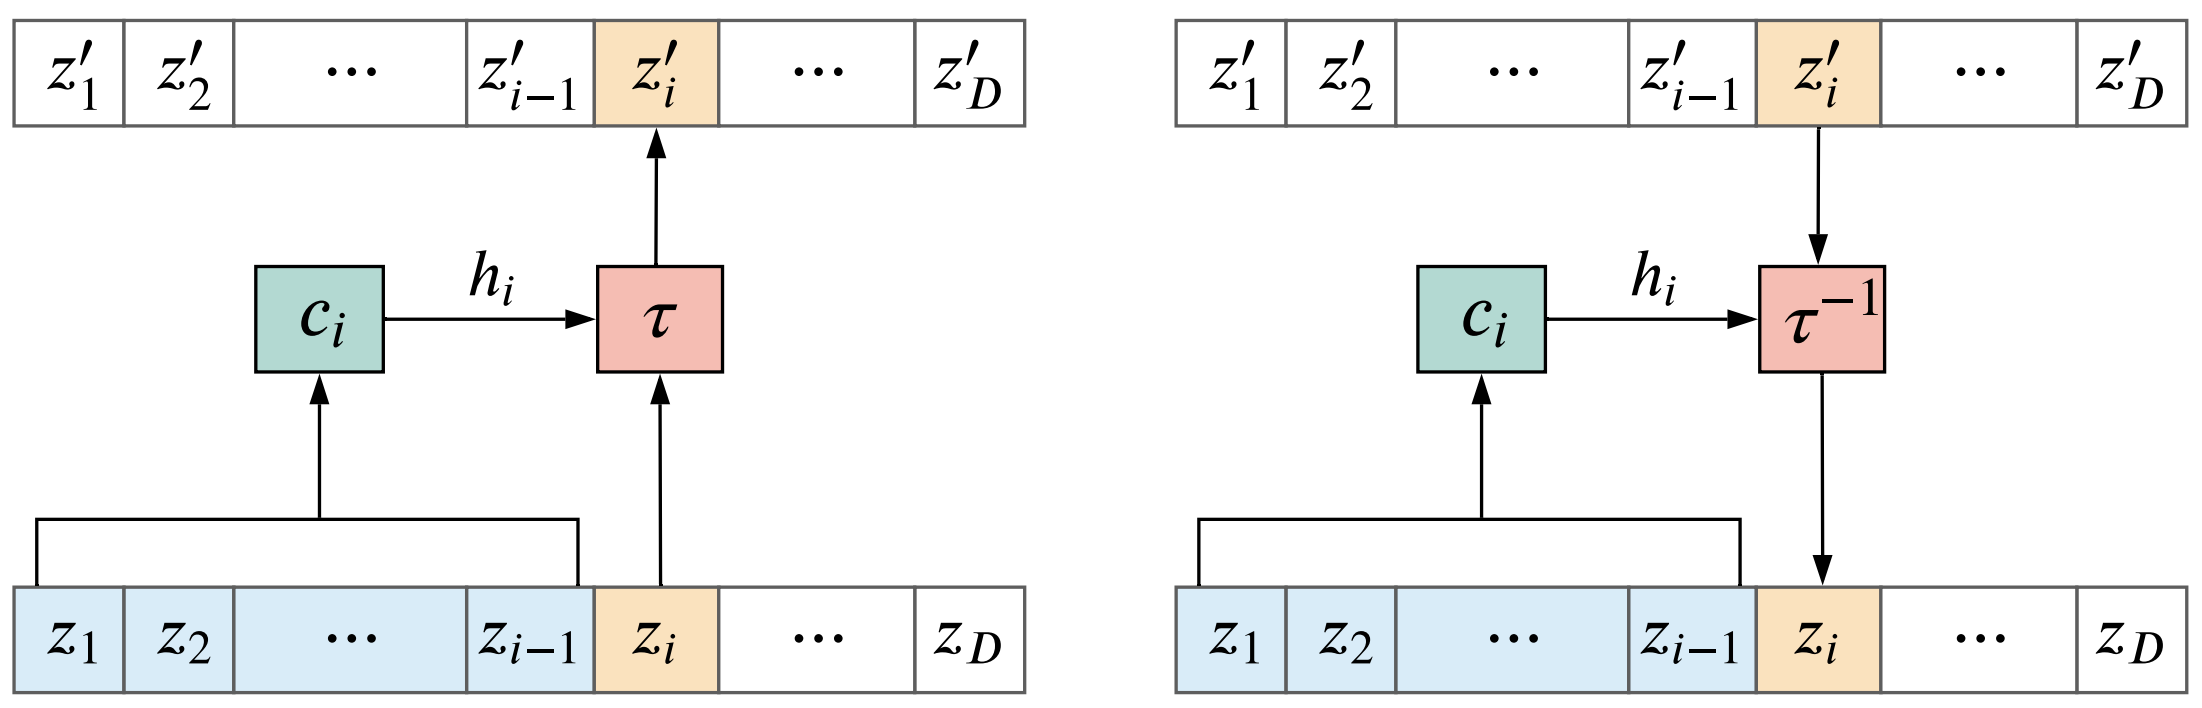
\includegraphics[width=0.9\linewidth]{figs/autoregressive_flow}
		\end{figure}
	\end{block}
	\begin{block}{RealNVP: Affine coupling law}
		\vspace{-0.7cm}
		\[
			\begin{cases} \bz_{1:d} = \bx_{1:d}; \\ \bz_{d:m} = \tau (\bx_{d:m}, c(\bx_{1:d}));\end{cases} 
			\quad \Leftrightarrow \quad 
			\begin{cases} \bx_{1:d} = \bz_{1:d}; \\ \bx_{d:m} = \tau^{-1} (\bz_{d:m}, c(\bz_{1:d})).\end{cases}
		\]
	\end{block}
	\myfootnote{
	\href{https://arxiv.org/abs/1410.8516}{Dinh L., Krueger D., Bengio Y. NICE: Non-linear Independent Components Estimation, 2014} \\
	\href{https://arxiv.org/abs/1605.08803}{Dinh L., Sohl-Dickstein J., Bengio S. Density estimation using Real NVP, 2016}}
\end{frame}
%=======
\begin{frame}{Linear flows}
	
	\begin{block}{RealNVP}
		\vspace{-0.5cm}
		\begin{equation*}
			\begin{cases} \bz_{1:d} = \bx_{1:d}; \\ \bz_{d:m} = \tau (\bx_{d:m}, c(\bx_{1:d}));\end{cases} 
			\quad \Leftrightarrow \quad 
			\begin{cases} \bx_{1:d} = \bz_{1:d}; \\ \bx_{d:m} = \tau^{-1} (\bz_{d:m}, c(\bz_{1:d})).\end{cases}
		\end{equation*}
		\vspace{-0.2cm}
	\end{block}
	\begin{itemize}
	\item First step is a \textbf{split} operator which decouples a variable into 2 subparts: $\bx_1$ and $\bx_2$ (usualy channel-wise).
	\item We should \textbf{permute} components between different layers.
	\end{itemize}
	\[
		\bz = \bW \bx, \quad \bW \in \bbR^{m \times m}
	\]
	In general, we need $O(m^3)$ to invert matrix.
	\begin{block}{Invertibility}
		\begin{itemize}
			\item Diagonal matrix $O(m)$.
			\item Triangular matrix $O(m^2)$.
			\item It is impossible to parametrize all invertible matrices.
		\end{itemize}
	\end{block}
\end{frame}
%=======
\begin{frame}{Linear flows}
	\vspace{-0.3cm}
	\[
		\bz = \bW \bx, \quad \bW \in \bbR^{m \times m}
	\]
	\vspace{-0.3cm}
	\begin{block}{Matrix decompositions}
		\begin{itemize}
			\item LU-decomposition
			\[
				\bW = \mathbf{P} \bL \bU,
			\]
			where $\mathbf{P}$ is a permutation matrix, $\mathbf{L}$ is lower triangular with positive diagonal, $\mathbf{U}$ is upper triangular with positive diagonal.
			\item QR-decomposition
			\[
				\bW = \bQ \mathbf{R},
			\]
			where $\bQ$ is an orthogonal matrix, $\mathbf{R}$ is an upper triangular matrix with positive diagonal.
		\end{itemize}
	\end{block}

	\myfootnote{
		\href{https://arxiv.org/abs/1807.03039}{Kingma D. P., Dhariwal P. Glow: Generative Flow with Invertible 1x1 Convolutions, 2018}  \\
		\href{https://arxiv.org/abs/1901.11137}{Hoogeboom E., Van Den Berg R., and Welling M. Emerging convolutions for generative normalizing flows, 2019}
	}
\end{frame}
%=======
\begin{frame}{Glow samples}
	\begin{figure}
		\centering
		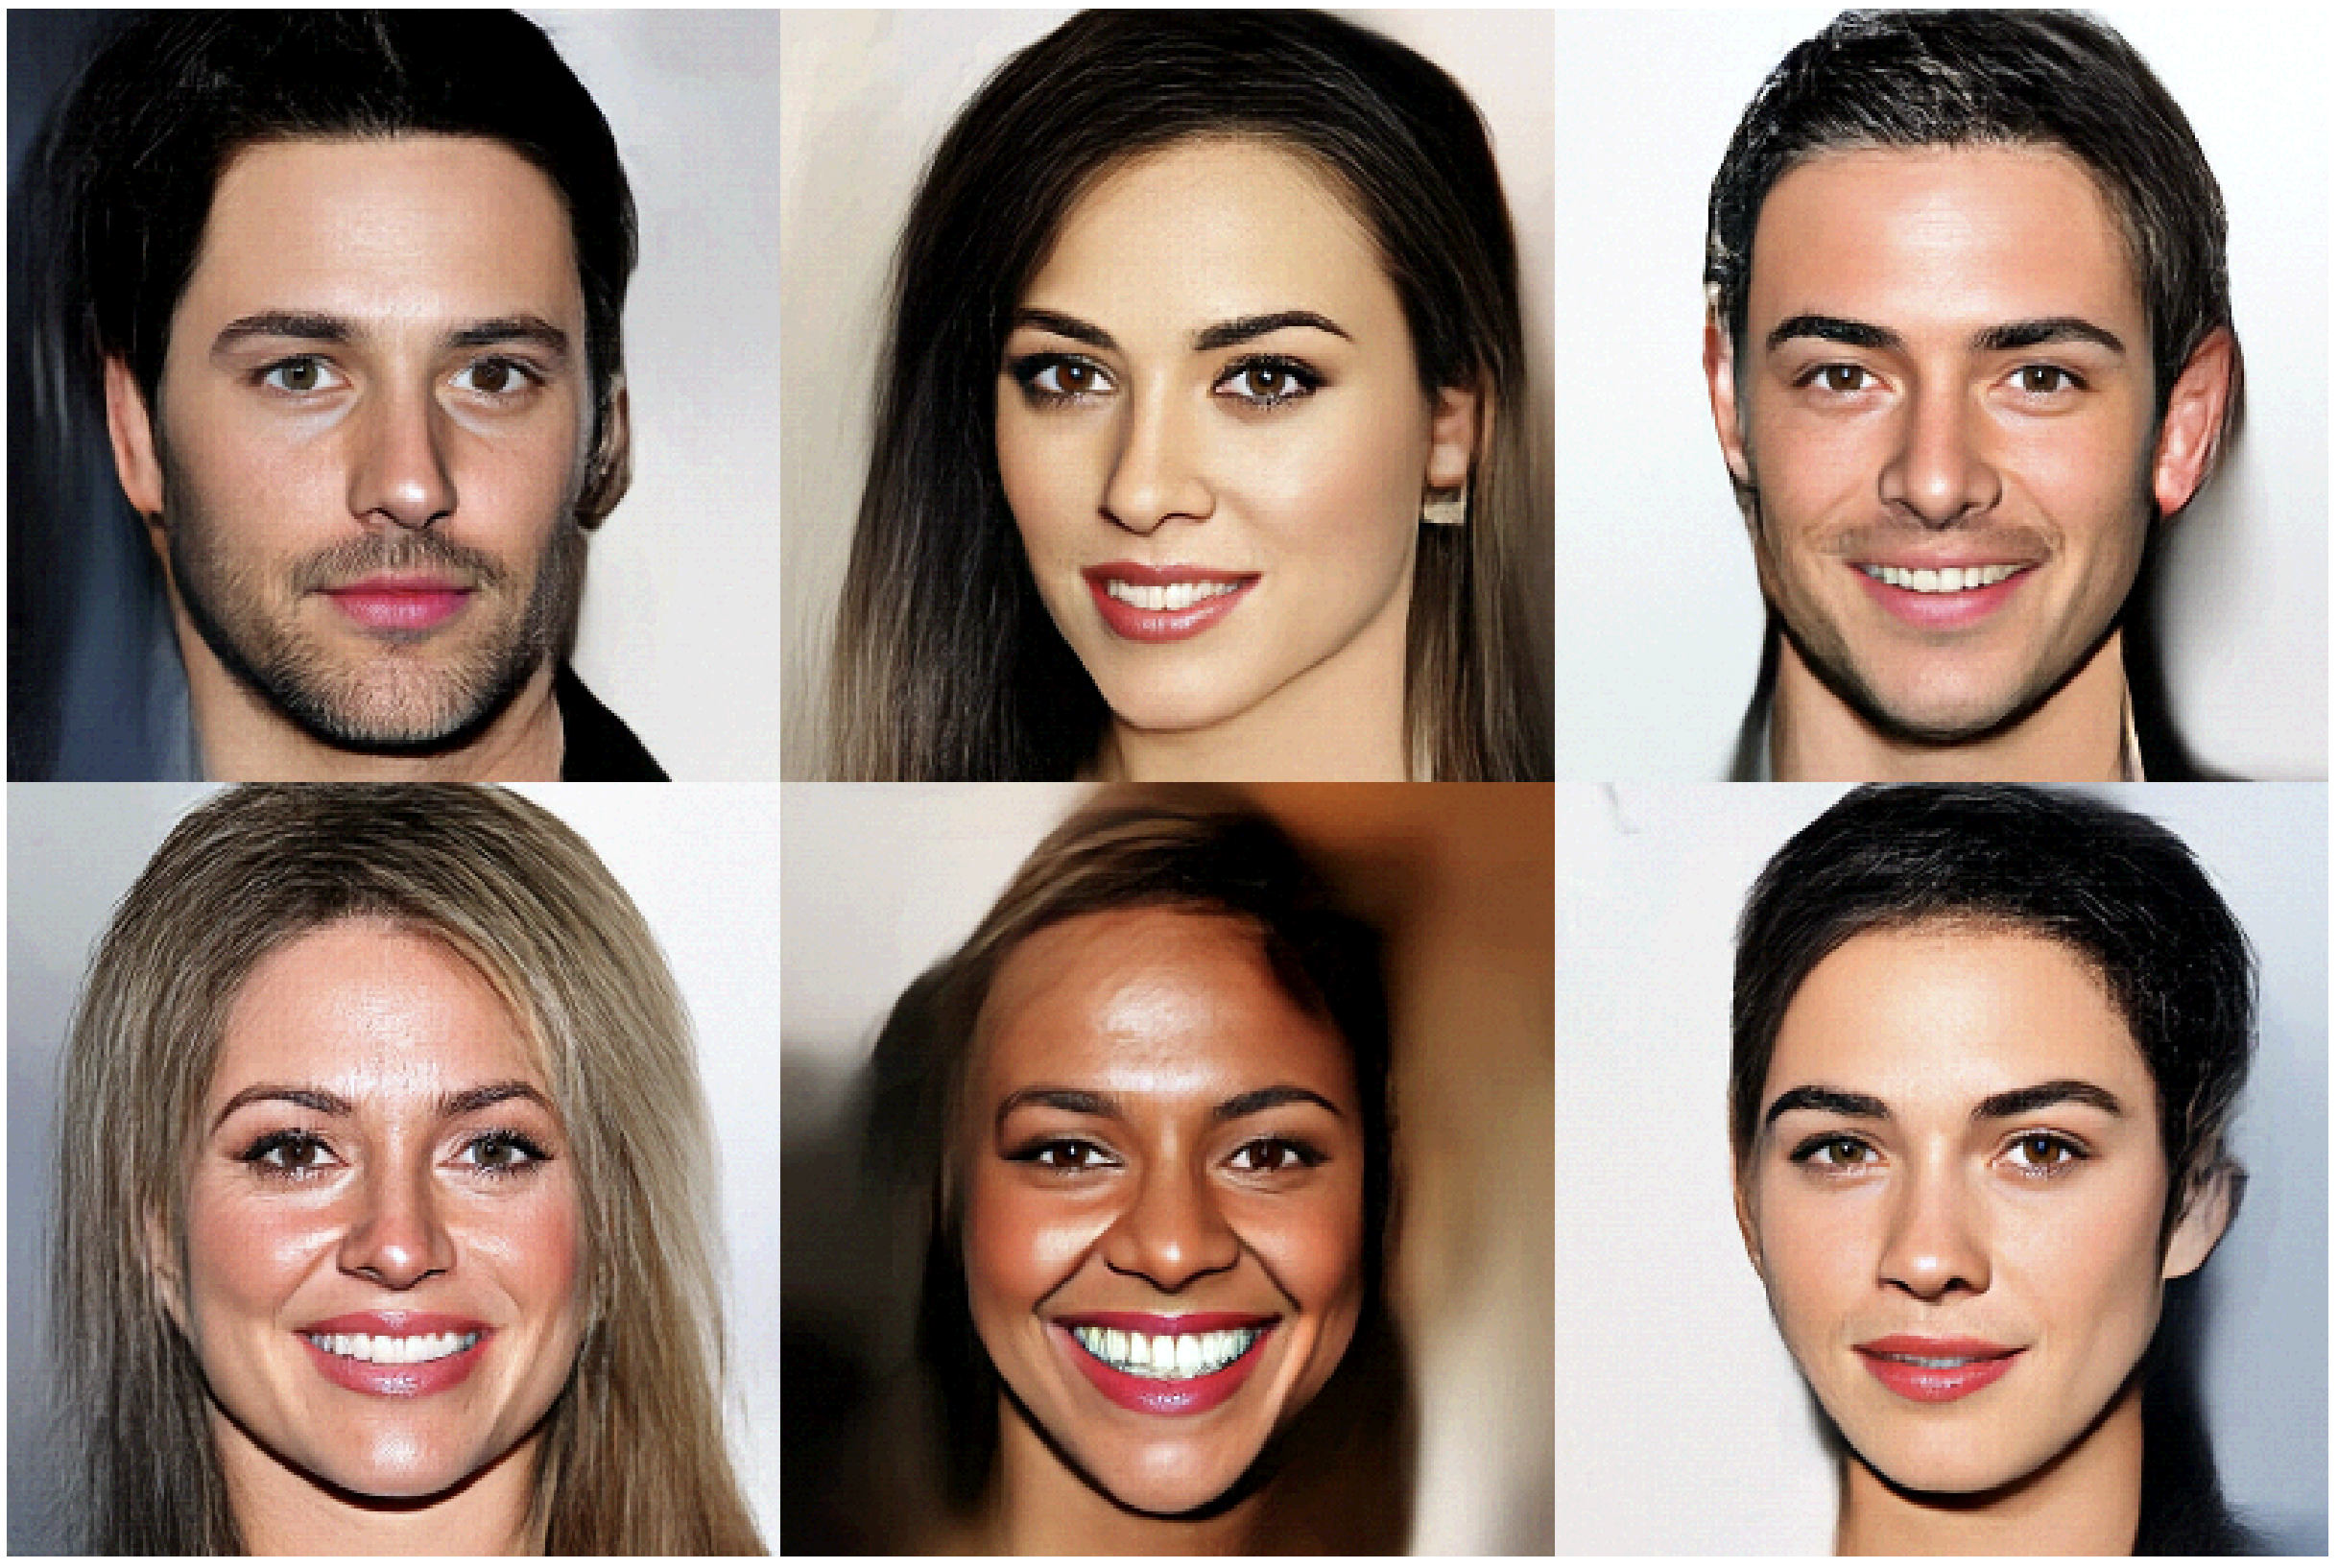
\includegraphics[width=\linewidth]{figs/glow_faces.png}
	\end{figure}
	\myfootnotewithlink{https://arxiv.org/abs/1807.03039}{Kingma D. P., Dhariwal P. Glow: Generative Flow with Invertible 1x1 Convolutions, 2018}
\end{frame}
%=======

\begin{frame}{MAF/IAF pros and cons}
	\begin{minipage}{0.50\columnwidth}
		\begin{block}{MAF}
			\begin{itemize}
				\item Sampling is slow.
				\item Likelihood evaluation is fast.
			\end{itemize}
		\end{block}
	\end{minipage}%
	\begin{minipage}{0.51\columnwidth}
		\begin{block}{IAF}
			\begin{itemize}
				\item Sampling is fast.
				\item Likelihood evaluation is slow.
			\end{itemize}
		\end{block}
	\end{minipage}
	How to take the best of both worlds?
	\begin{block}{WaveNet}
		Autoregressive model with caused dilated convolutions for raw audio waveforms generation.
		\vspace{-0.5cm}
		\[
			p(\bx| \btheta) = \prod_{t=1}^T p(x_t|\bx_{1:t-1}, \btheta).
		\]
		\vspace{-0.7cm}
		\begin{figure}
			\centering
			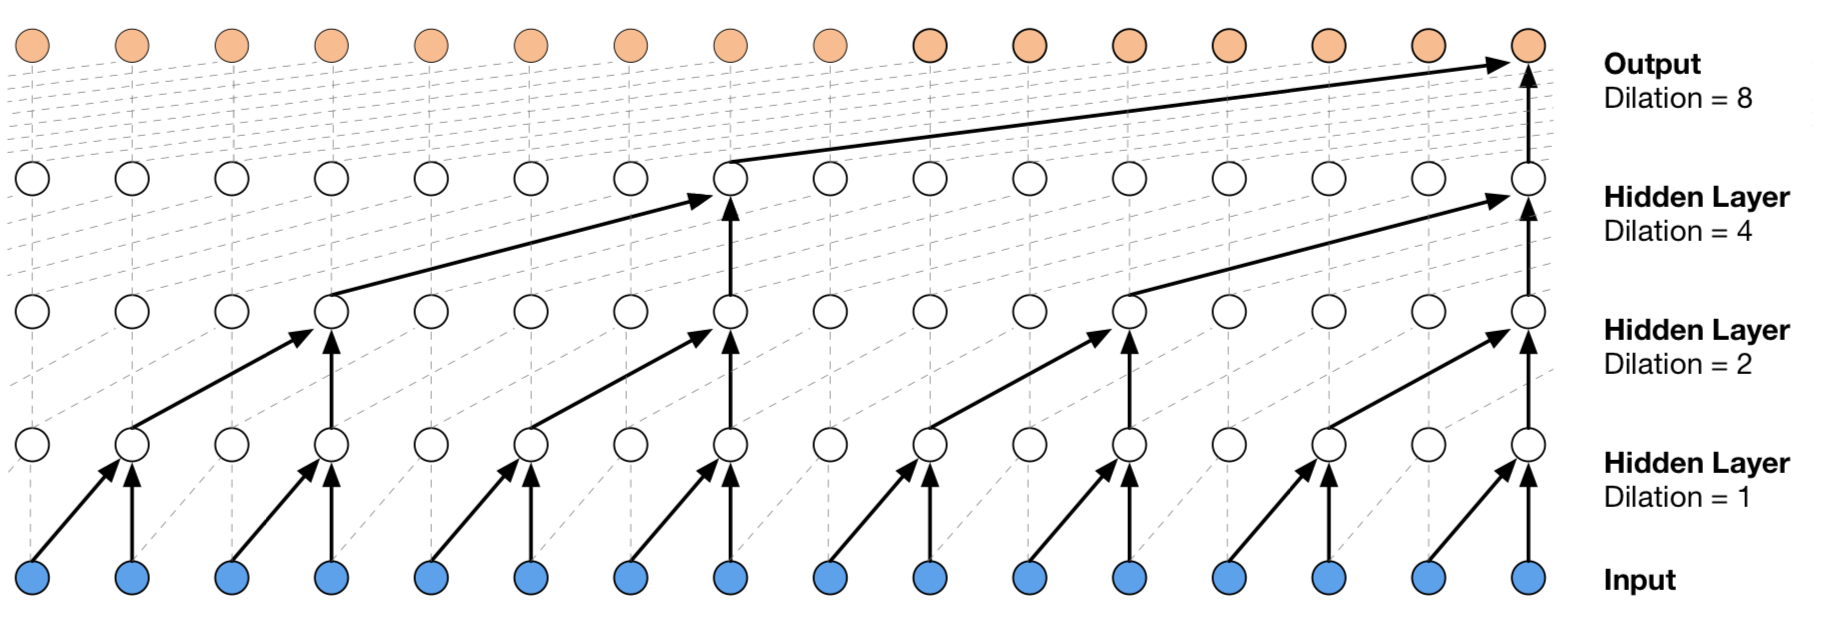
\includegraphics[width=0.85\linewidth]{figs/wavenet2.png}
		\end{figure}
	\end{block}
	\myfootnotewithlink{https://arxiv.org/abs/1609.03499}{Oord A. et al. Wavenet: A generative model for raw audio, 2016}
\end{frame}
%=======
\begin{frame}{Parallel WaveNet}
	\begin{itemize}
		\item 24kHz instead of 16kHz using increased dilated convolution filter size from 2 to 3.
		\item 16-bit signals with mixture of logistics instead of 8-bit signal with 256-way categorical distribution.
	\end{itemize}
	\begin{block}{Probability density distillation}
		\begin{enumerate}
			\item Train usual WaveNet (MAF) via MLE (teacher network).
			\item Train IAF WaveNet (student network), which attempts to match the probability of its own samples under the distribution learned by the teacher.
		\end{enumerate}
	\end{block}
	\vspace{-0.3cm}
	\begin{block}{Student objective}
		\vspace{-0.3cm}
		\[
			KL(p_s || p_t) = H(p_s, p_t) - H(p_s).
		\]
		\vspace{-0.3cm}
	\end{block}
	More than 1000x speed-up relative to original WaveNet!
	\myfootnotewithlink{https://arxiv.org/abs/1711.10433}{Oord A. et al. Parallel WaveNet: Fast High-Fidelity Speech Synthesis, 2017}
\end{frame}
%=======
\begin{frame}{Parallel WaveNet}
	\begin{figure}
		\centering
		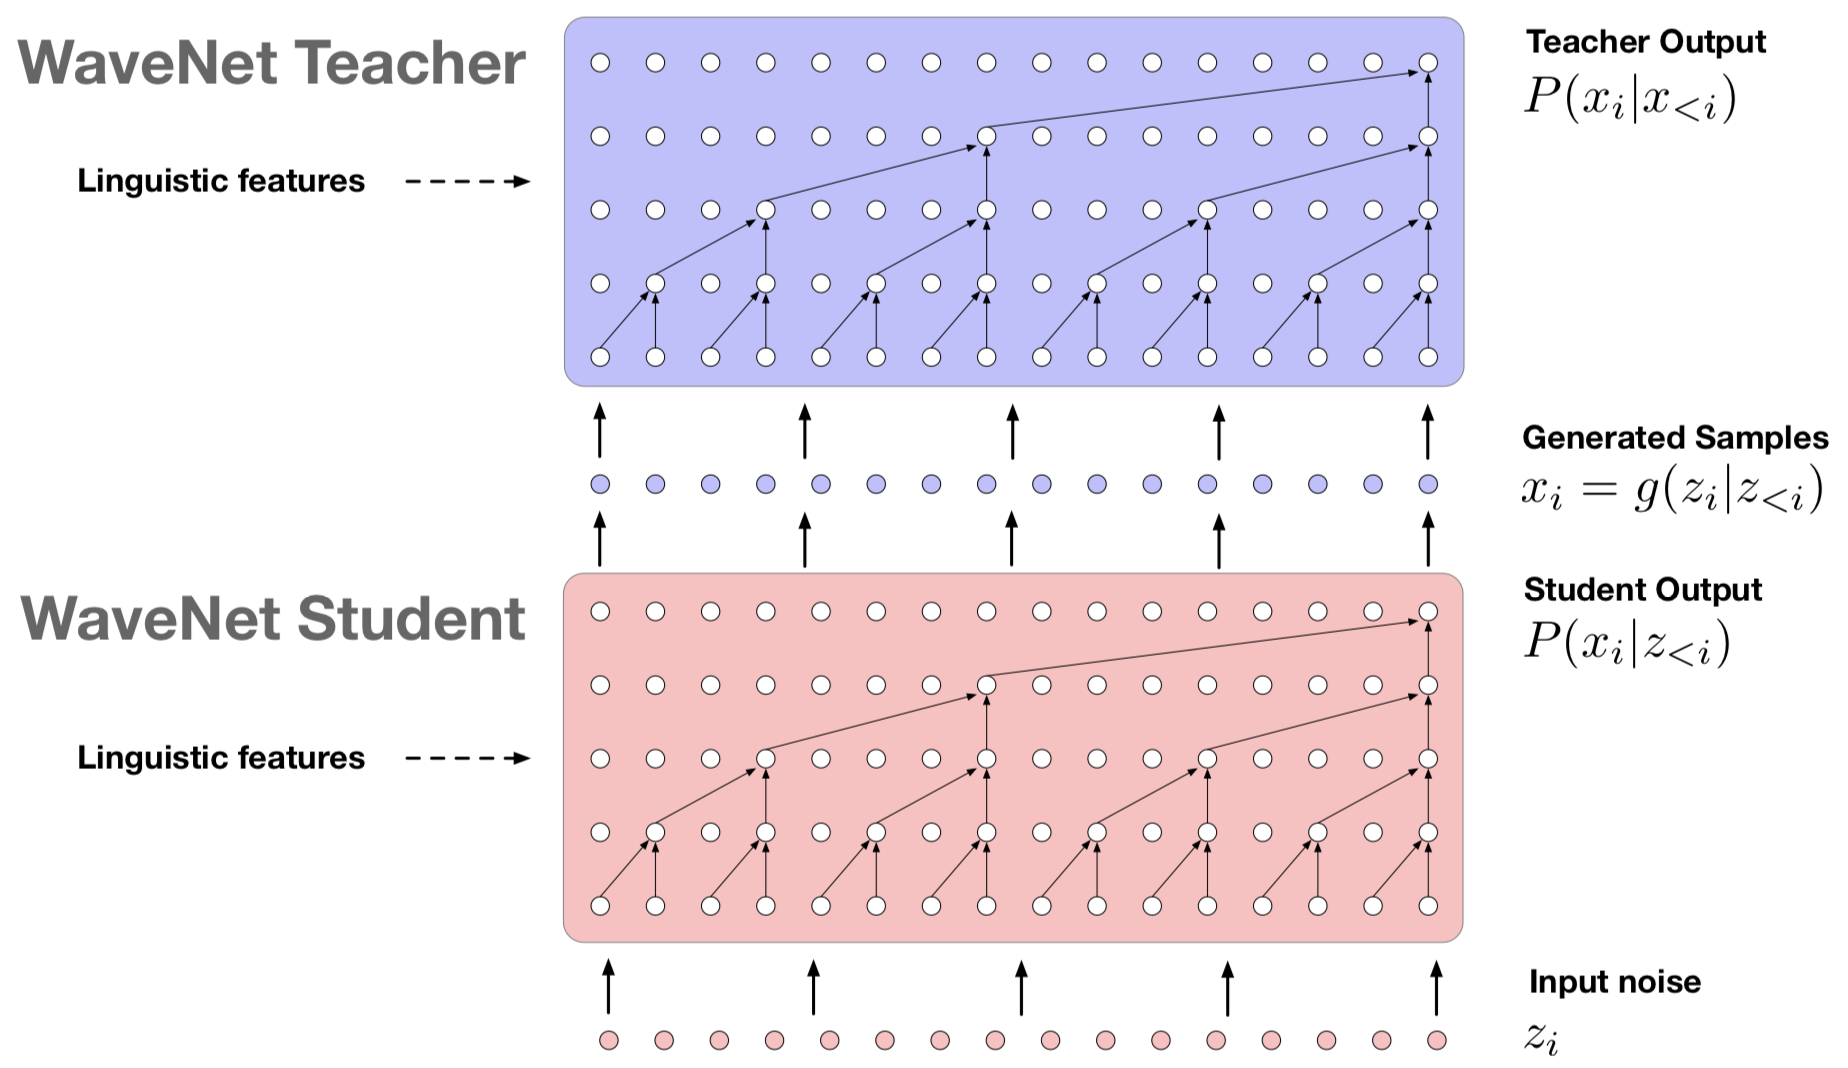
\includegraphics[width=\linewidth]{figs/parallel_wavenet.png}
	\end{figure}

	\myfootnotewithlink{https://arxiv.org/abs/1711.10433}{Oord A. et al. Parallel WaveNet: Fast High-Fidelity Speech Synthesis, 2017}
\end{frame}
%=======
\begin{frame}{Likelihood-based models}
\begin{block}{Exact likelihood evaluation}
	\begin{itemize}
		\item Autoregressive models (PixelCNN, WaveNet);
		\item Flow models (NICE, RealNVP, Glow).
	\end{itemize}
\end{block}
\begin{block}{Approximate likelihood evaluation}
	\begin{itemize}
		\item Latent variable models (VAE).
	\end{itemize}
\end{block}
What are the pros and cons of each of them? \\
\vspace{0.2cm}
\end{frame}
%=======
\begin{frame}{VAE recap}
\begin{block}{ELBO}
	\vspace{-0.3cm}
	\[
	\log p(\bx | \btheta) \geq \mathcal{L} (\bphi, \btheta)  = \mathbb{E}_{q(\bz | \bx, \bphi)} \log \frac{p(\bx, \bz | \btheta)}{q(\bz| \bx, \bphi)} \rightarrow \max_{\bphi, \btheta}.
	\]
	\vspace{-0.5cm}
\end{block}
\begin{figure}[h]
	\centering
	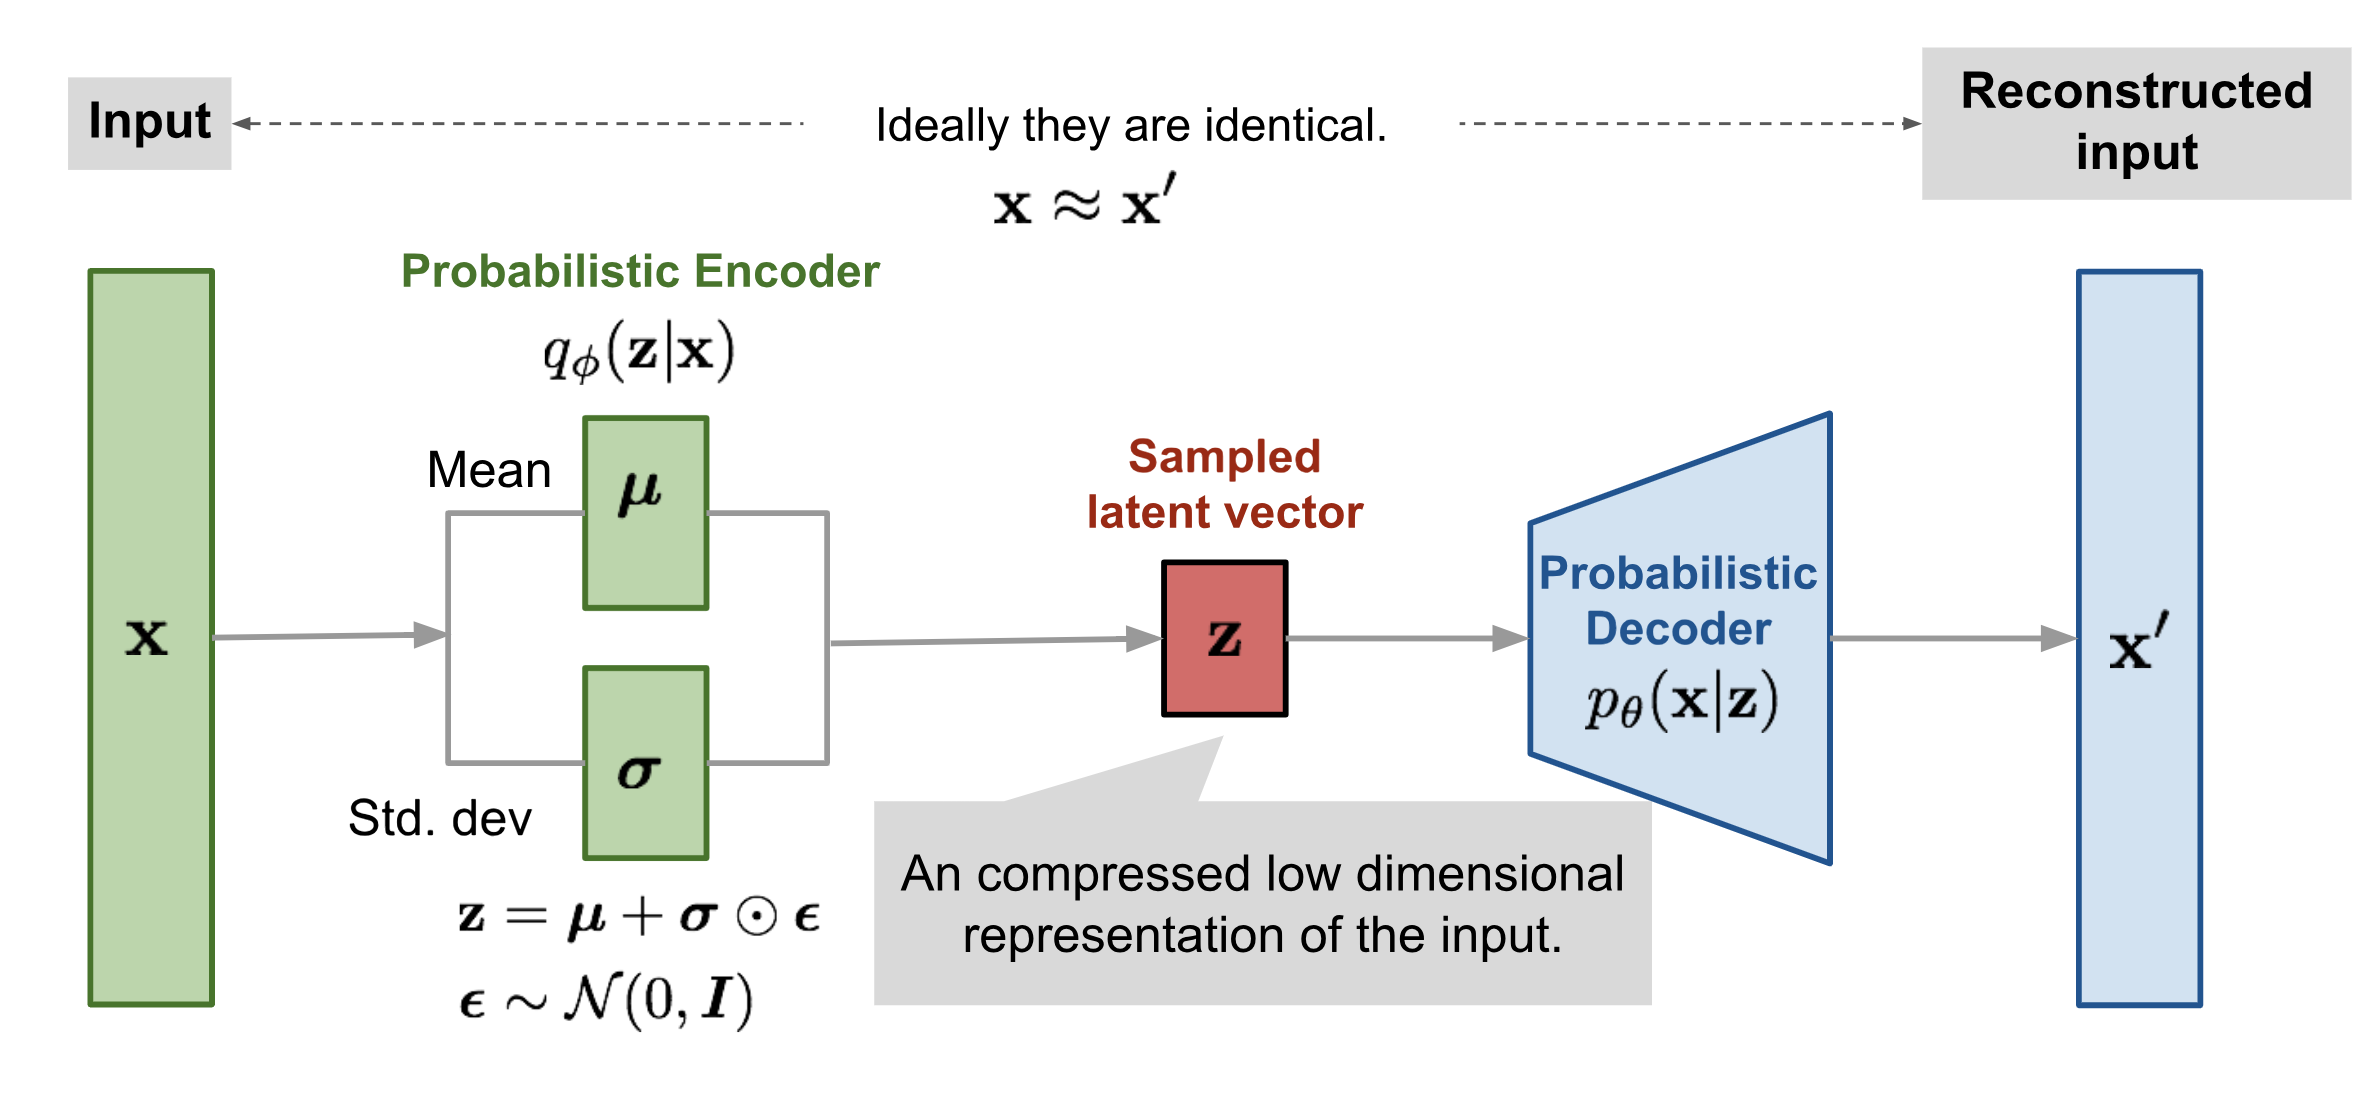
\includegraphics[width=\linewidth]{figs/vae-gaussian.png}
\end{figure}
\myfootnotewithlink{https://lilianweng.github.io/lil-log/2018/08/12/from-autoencoder-to-beta-vae.html}{image credit: https://lilianweng.github.io/lil-log/2018/08/12/from-autoencoder-to-beta-vae.html}

\end{frame}
%=======
\begin{frame}{VAE limitations}
\begin{itemize}
	\item Poor variational posterior distribution (encoder)
	\[
	q(\bz | \bx, \bphi) = \mathcal{N}(\bz| \bmu_{\bphi}(\bx), \bsigma^2_{\bphi}(\bx)).
	\]
	\item Poor prior distribution
	\[
	p(\bz) = \mathcal{N}(0, \mathbf{I}).
	\]
	\item Poor probabilistic model (decoder)
	\[
	p(\bx | \bz, \btheta) = \mathcal{N}(\bx| \bmu_{\btheta}(\bz), \bsigma^2_{\btheta}(\bz)) \quad (\text{or } \text{Softmax}(\pi(\bz))).
	\]
	\item Loose lower bound
	\[
	\log p(\bx | \btheta) - \mathcal{L}(q, \btheta) = (?).
	\]
\end{itemize}
\end{frame}
%=======
\begin{frame}{Posterior collapse}
	\begin{block}{Representation learning}
		"Identifies and disentangles the underlying causal factors of the data, so that it becomes easier to understand the data, to classify it, or to perform other tasks".
	\end{block}
	\vspace{-0.2cm}
	\[
		p(\bx | \btheta) = \int p(\bx, \bz | \btheta) d \bz = \int p(\bx | \bz, \btheta) p(\bz) d \bz 
	\]
	If the decoder model $p(\bx | \bz, \btheta)$ is powerful enough to model $p(\bx | \btheta)$ the latent variables $\bz$ becomes irrelevant.
	\[
		\mathcal{L}(q, \btheta) = \left[ \mathbb{E}_{q(\bz | \bx)} \log p(\bx | \bz, \btheta) - KL(q(\bz | \bx) || p(\bz)) \right].
	\]
	Early in the training the approximate posterior $q(\bz|\bx)$ carries little information about $\bx$ and the model sets the posterior to the prior to avoid paying any cost $KL(q(\bz|\bx)||p(\bz))$.
\end{frame}
%=======
\begin{frame}{PixelVAE}
	\begin{block}{LVM}
		\vspace{-0.3cm}
		\[
		    p(\bx | \btheta) = \int p(\bx, \bz | \btheta) d \bz = \int p(\bx | \bz, \btheta) p(\bz) d \bz 
		\]
		\vspace{-0.3cm}
	\end{block}
	\begin{itemize}
		\item More powerful $p(\bx | \bz, \btheta)$ leads to more powerful generative model $p(\bx | \btheta)$.
		\item Too powerful $p(\bx | \bz, \btheta)$ could lead to posterior collapse, where variational posterior $q(\bz | \bx)$ will not carry any information about data and close to prior $p(\bz)$.
	\end{itemize}
	How to make the generative model $p(\bx | \bz, \btheta)$ more powerful?
	\begin{block}{Autoregressive decoder}
		\vspace{-0.2cm}
		\[
		    p(\bx | \bz , \btheta) = \prod_{i=1}^n p(x_i | \bx_{1:i - 1}, \bz , \btheta)
		\]
	\end{block}
	
	\myfootnotewithlink{https://arxiv.org/abs/1611.05013}{Gulrajani I. et al. PixelVAE: A Latent Variable Model for Natural Images, 2016}
\end{frame}
%=======
\begin{frame}{PixelVAE}
	\begin{block}{Autoregressive decoder}
		\vspace{-0.3cm}
		\[
		p(\bx | \bz , \btheta) = \prod_{i=1}^n p(x_i | \bx_{1:i - 1}, \bz , \btheta)
		\]
		\vspace{-0.3cm}
	\end{block}
	\begin{itemize}
		\item Global structure is captured by latent variables.
		\item Local statistics are captured by limited receptive field autoregressive model.
	\end{itemize}
	\vspace{-0.1cm}
	\begin{block}{MNIST results}
		\vspace{-0.3cm}
		\begin{figure}
		    \centering
		    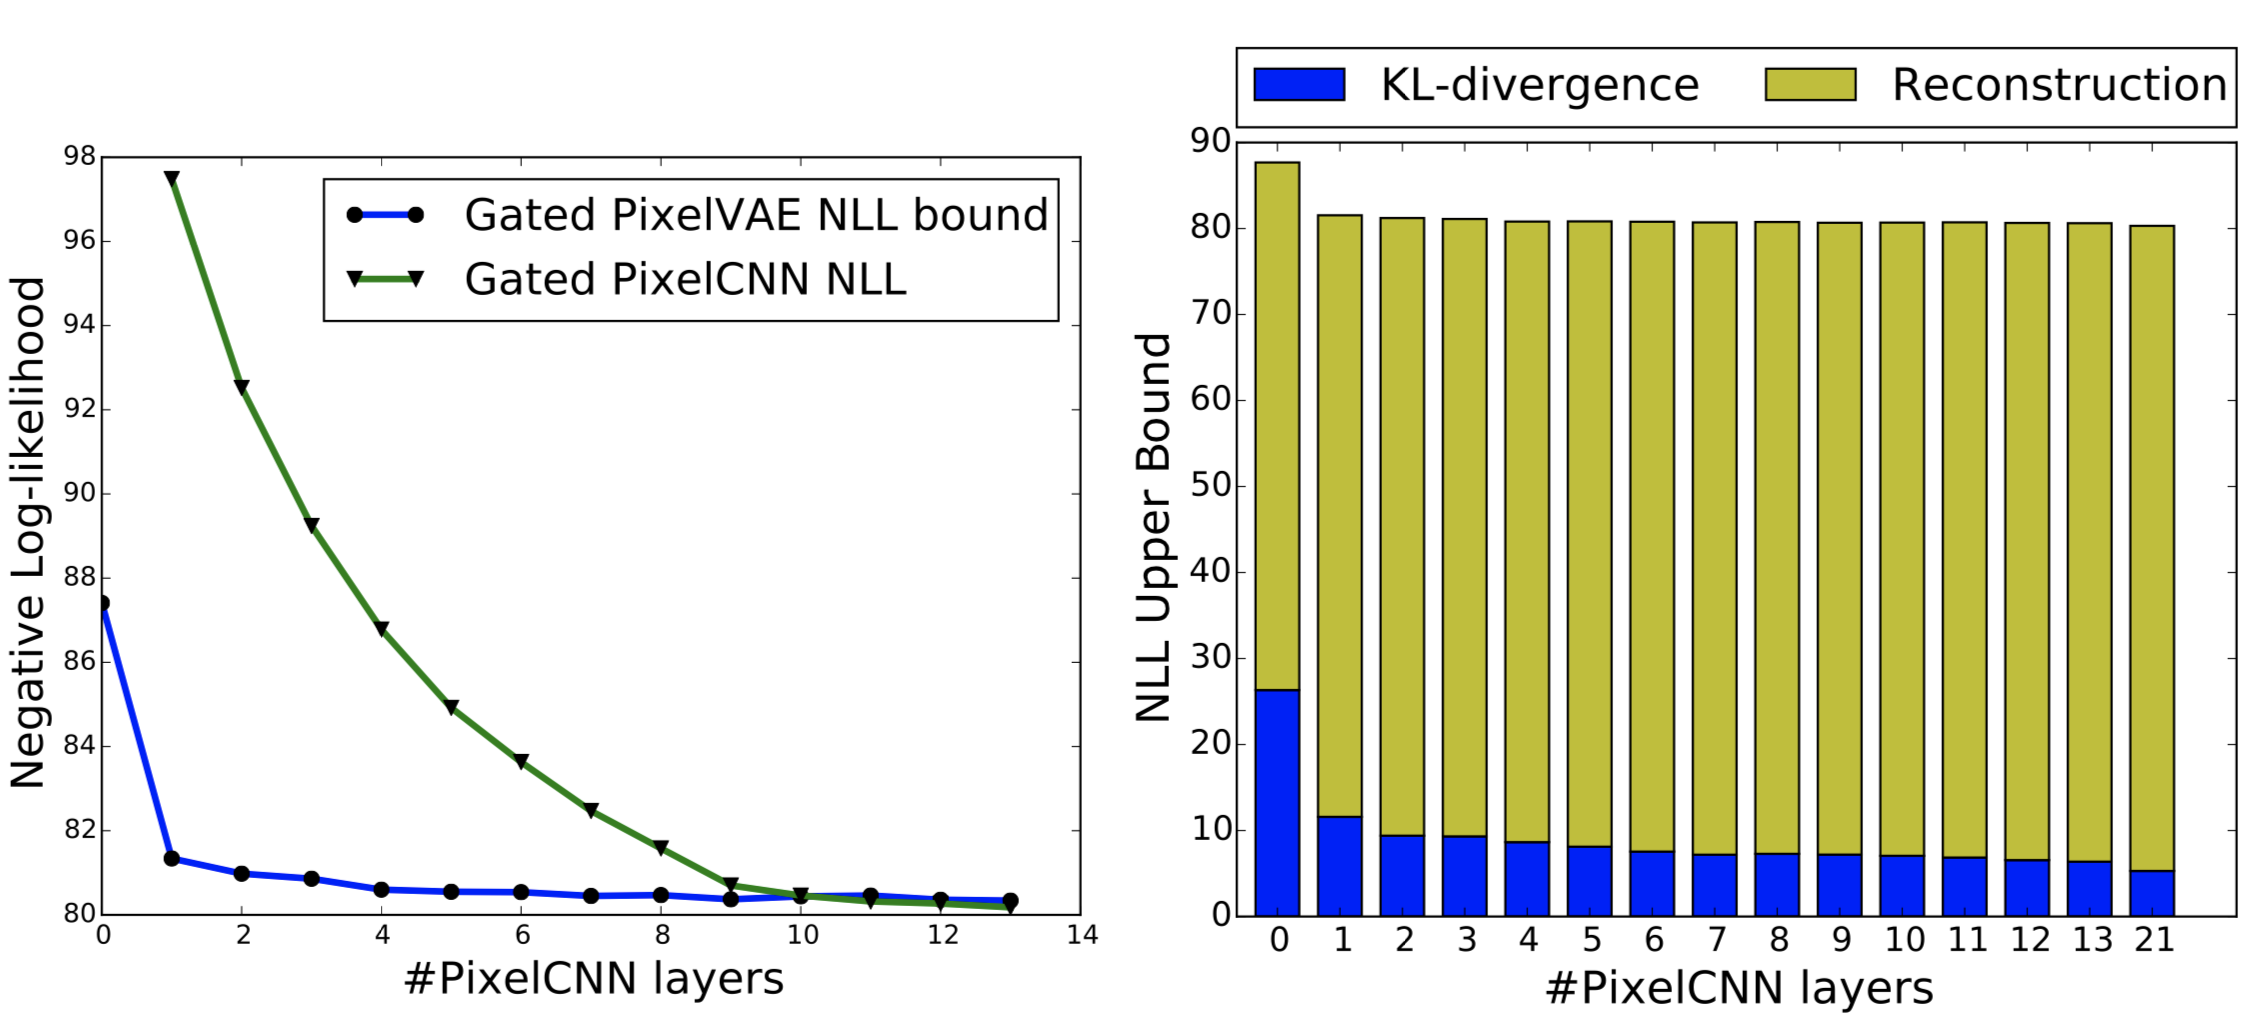
\includegraphics[width=0.75\linewidth]{figs/PixelVAE_2.png}
		\end{figure}
	\end{block}
		
	\myfootnotewithlink{https://arxiv.org/abs/1611.05013}{Gulrajani I. et al. PixelVAE: A Latent Variable Model for Natural Images, 2016}
\end{frame}
%=======
\begin{frame}{Decoder weakening}
	\begin{itemize}
		\item Powerful decoder $p(\bx | \bz, \btheta)$ makes the model expressive, but posterior collapse is possible.
		\item PixelVAE model uses the autoregressive PixelCNN model with small number of layers to limit receptive field.
	\end{itemize}
	How to force the model encode information about $\bx$ into $\bz$?
	\begin{block}{KL annealing}
		\vspace{-0.3cm}
		\[
		    \mathcal{L}(q, \btheta, \beta) = \mathbb{E}_{q(\bz | \bx)} \log p(\bx | \bz, \btheta) - \beta \cdot KL (q(\bz | \bx) || p(\bz))
		\]
		Start training with $\beta = 0$, increase it until $\beta = 1$ during training.
	\end{block}
	\vspace{-0.2cm}
	\begin{block}{Free bits}
		\vspace{-0.7cm}
		\[
		    \mathcal{L}(q, \btheta, \lambda) = \mathbb{E}_{q(\bz | \bx)} \log p(\bx | \bz, \btheta) - \max(\lambda, KL (q(\bz | \bx) || p(\bz))).
		\]
		\vspace{-0.7cm} \\
		It ensures the use of less than $\lambda$ bits of information and results in $KL (q(\bz | \bx) || p(\bz)) \geq \lambda$.
	\end{block}
	\myfootnote{\href{https://arxiv.org/abs/1511.06349}{Bowman S. R. et al. Generating Sentences from a Continuous Space, 2015} \\
	\href{https://arxiv.org/abs/1606.04934}{Kingma D. P. et al. Improving Variational Inference with Inverse Autoregressive Flow, 2016}}
\end{frame}
%=======
\begin{frame}{VAE limitations}
	\begin{itemize}
		\item Poor variational posterior distribution (encoder)
		\[
		q(\bz | \bx, \bphi) = \mathcal{N}(\bz| \bmu_{\bphi}(\bx), \bsigma^2_{\bphi}(\bx)).
		\]
		\item Poor prior distribution
		\[
		p(\bz) = \mathcal{N}(0, \mathbf{I}).
		\]
		\item Poor probabilistic model (decoder)
		\[
		p(\bx | \bz, \btheta) = \mathcal{N}(\bx| \bmu_{\btheta}(\bz), \bsigma^2_{\btheta}(\bz)).
		\]
		\item Loose lower bound
		\[
		\log p(\bx | \btheta) - \mathcal{L}(q, \btheta) = (?).
		\]
	\end{itemize}
\end{frame}
%=======
\begin{frame}{Importance Sampling}
	\begin{block}{Generative model}
		\vspace{-0.5cm}
		\begin{align*}
			p(\bx | \btheta) &= \int p(\bx, \bz | \btheta) d\bz = \int \left[\frac{p(\bx, \bz | \btheta)}{q(\bz | \bx)} \right] q(\bz | \bx) d\bz \\
			&= \int f(\bx, \bz) q(\bz | \bx) d\bz = \mathbb{E}_{\bz \sim q(\bz | \bx)} f(\bx, \bz)
		\end{align*}
	\end{block}
	Here $f(\bx, \bz) = \frac{p(\bx, \bz | \btheta)}{q(\bz | \bx)}$.
	\begin{block}{ELBO}
		\vspace{-0.5cm}
		\begin{multline*}
			\log p(\bx | \btheta) = \log \mathbb{E}_{\bz \sim q(\bz | \bx)} f(\bx, \bz)
			\geq \mathbb{E}_{\bz \sim q(\bz | \bx)} \log f(\bx, \bz) = \\
			= \mathbb{E}_{\bz \sim q(\bz | \bx)} \log \frac{p(\bx, \bz | \btheta)}{q(\bz | \bx)} = \mathcal{L}(q, \btheta).
		\end{multline*}
	\end{block}
	Could we choose better $f(\bx, \bz)$? 
\end{frame}
%=======
\begin{frame}{IWAE}
		\[
			p(\bx | \btheta) = \int p(\bx, \bz | \btheta) d\bz = \int \left[\frac{p(\bx, \bz | \btheta)}{q(\bz | \bx)} \right] q(\bz | \bx) d\bz = \mathbb{E}_{\bz \sim q(\bz | \bx)} f(\bx, \bz)
		\]
	Let define
	\[
	f(\bx, \bz_1, \dots, \bz_K) = \frac{1}{K} \sum_{k=1}^K \frac{p(\bx, \bz_k | \btheta)}{q(\bz_k | \bx)}
	\]
	\[
		\mathbb{E}_{\bz_1, \dots, \bz_K \sim q(\bz | \bx)} f(\bx, \bz_1, \dots, \bz_K) = p(\bx | \btheta)
	\]
	\vspace{-0.3cm}
	\begin{block}{ELBO}
		\vspace{-0.5cm}
		\begin{multline*}
			\log p(\bx | \btheta) = \log \mathbb{E}_{\bz_1, \dots, \bz_K \sim q(\bz | \bx)} f(\bx, \bz, \dots, \bz_K) \geq \\
			\geq \mathbb{E}_{\bz_1, \dots, \bz_K \sim q(\bz | \bx)} \log f(\bx, \bz, \dots, \bz_K) = \\
			= \mathbb{E}_{\bz_1, \dots, \bz_K \sim q(\bz | \bx)} \log \left[\frac{1}{K} \sum_{k=1}^K\frac{p(\bx, \bz_k | \btheta)}{q(\bz_k | \bx)} \right] = \mathcal{L}_K(q, \btheta).
		\end{multline*}
	\end{block}
	\myfootnotewithlink{https://arxiv.org/abs/1509.00519}{Burda Y., Grosse R., Salakhutdinov R. Importance Weighted Autoencoders, 2015}
\end{frame}
%=======
\begin{frame}{IWAE}
	\begin{block}{VAE objective}
		\vspace{-0.2cm}
		\[
		\log p(\bx | \btheta) \geq \mathcal{L} (q, \btheta)  = \mathbb{E}_{q(\bz | \bx)} \log \frac{p(\bx, \bz | \btheta)}{q(\bz| \bx)} \rightarrow \max_{q, \btheta}
		\]
		\[
		\mathcal{L} (q, \btheta)  = \mathbb{E}_{\bz_1, \dots, \bz_K \sim q(\bz | \bx)} \left( \frac{1}{K} \sum_{k=1}^K \log \frac{p(\bx, \bz_k | \btheta)}{q(\bz_k| \bx)} \right) \rightarrow \max_{q, \btheta}.
		\]
		\vspace{-0.2cm}
	\end{block}
	\begin{block}{IWAE objective}
		\vspace{-0.2cm}
		\[
		\mathcal{L}_K (q, \btheta)  = \mathbb{E}_{\bz_1, \dots, \bz_K \sim q(\bz | \bx)} \log \left( \frac{1}{K}\sum_{k=1}^K\frac{p(\bx, \bz_k | \btheta)}{q(\bz_k| \bx)} \right) \rightarrow \max_{q, \btheta}.
		\]
	\end{block}
	If $K=1$, these objectives coincide.

	\myfootnotewithlink{https://arxiv.org/abs/1509.00519}{Burda Y., Grosse R., Salakhutdinov R. Importance Weighted Autoencoders, 2015}
\end{frame}
%=======
\begin{frame}{IWAE}
	\begin{block}{Theorem}
		\begin{enumerate}
			\item $\log p(\bx | \btheta) \geq \mathcal{L}_K (q, \btheta) \geq \mathcal{L}_M (q, \btheta), \quad \text{for } K \geq M$;
			\item $\log p(\bx | \btheta) = \lim_{K \rightarrow \infty} \mathcal{L}_K (q, \btheta)$ if $\frac{p(\bx, \bz | \btheta)}{q(\bz | \bx)}$ is bounded.
		\end{enumerate}
		\vspace{-0.2cm}
	\end{block}
	\begin{block}{Proof of 1.}
		{ \footnotesize
			\vspace{-0.5cm}
			\begin{align*}
				\mathcal{L}_K (q, \btheta) &= \mathbb{E}_{\bz_1, \dots, \bz_K} \log \left( \frac{1}{K}\sum_{k=1}^K\frac{p(\bx, \bz_k | \btheta)}{q(\bz_k| \bx)} \right) = \\
				&= \mathbb{E}_{\bz_1, \dots, \bz_K} \log \mathbb{E}_{k_1, \dots, k_M} \left( \frac{1}{M}\sum_{m=1}^M\frac{p(\bx, \bz_{k_m} | \btheta)}{q(\bz_{k_m}| \bx)} \right) \geq \\
				&\geq \mathbb{E}_{\bz_1, \dots, \bz_K} \mathbb{E}_{k_1, \dots, k_m} \log \left( \frac{1}{M}\sum_{m=1}^M\frac{p(\bx, \bz_{k_m} | \btheta)}{q(\bz_{k_m}| \bx)} \right) = \\
				&= \mathbb{E}_{\bz_1, \dots, \bz_M} \log \left( \frac{1}{M}\sum_{m=1}^M\frac{p(\bx, \bz_m | \btheta)}{q(\bz_m| \bx)} \right) = \mathcal{L}_M (q, \btheta)
			\end{align*}
			\[
			\frac{a_1 + \dots + a_K}{K} = \mathbb{E}_{k_1, \dots, k_M} \frac{a_{k_1} + \dots + a_{k_M}}{M}, \quad k_1, \dots, k_M \sim U[1, K]
			\]
		}
	\end{block}
	
	\myfootnotewithlink{https://arxiv.org/abs/1509.00519}{Burda Y., Grosse R., Salakhutdinov R. Importance Weighted Autoencoders, 2015}
\end{frame}
%=======
\begin{frame}{IWAE}
	\begin{block}{Theorem}
		\begin{enumerate}
			\item $\log p(\bx | \btheta) \geq \mathcal{L}_K (q, \btheta) \geq \mathcal{L}_M (q, \btheta), \quad \text{for} K \geq M$;
			\item $\log p(\bx | \btheta) = \lim_{K \rightarrow \infty} \mathcal{L}_K (q, \btheta)$ if $\frac{p(\bx, \bz | \btheta)}{q(\bz | \bx)}$ is bounded.
		\end{enumerate}
		\vspace{-0.2cm}
	\end{block}
	\begin{block}{Proof of 2.}
		\vspace{0.2cm}
		Consider r.v. $\xi_K = \frac{1}{K}\sum_{k=1}^K \frac{p(\bx, \bz_k | \btheta)}{q(\bz_k | \bx)}$. \\
		\vspace{0.2cm}
		If summands are bounded, then (from the strong law of large numbers)
		\[
		\xi_K \xrightarrow[K \rightarrow \infty]{a.s.} \mathbb{E}_{q(\bz | \bx)} \frac{p(\bx, \bz | \btheta)}{q(\bz | \bx)} = p(\bx | \btheta).
		\]
		Hence $\mathcal{L}_K (q, \btheta) = \mathbb{E} \log \xi_K$ converges to $\log p(\bx | \btheta)$ as $K \rightarrow \infty$.
	\end{block}

	\myfootnotewithlink{https://arxiv.org/abs/1509.00519}{Burda Y., Grosse R., Salakhutdinov R. Importance Weighted Autoencoders, 2015}
\end{frame}
%=======
\begin{frame}{IWAE}
	\[
	\log p(\bx | \btheta) \geq \mathcal{L}_K(q, \btheta) \geq \mathcal{L}(q, \btheta)
	\]
	If $K > 1$ the bound could be tighter.
	\begin{align*}
		\mathcal{L} (q, \btheta) &= \mathbb{E}_{q(\bz | \bx)} \log \frac{p(\bx, \bz | \btheta)}{q(\bz| \bx)}; \\
		\mathcal{L}_K (q, \btheta) &= \mathbb{E}_{\bz_1, \dots, \bz_K \sim q(\bz | \bx)} \log \left( \frac{1}{K}\sum_{k=1}^K\frac{p(\bx, \bz_k | \btheta)}{q(\bz_k| \bx)} \right).
	\end{align*}
	\vspace{-0.2cm}
	\begin{itemize}
		\item $\mathcal{L}_1(q, \btheta) = \mathcal{L}(q, \btheta)$;
		\item $\mathcal{L}_{\infty}(q, \btheta) = \log p(\bx | \btheta)$.
		\item Which $q^*(\bz | \bx)$ gives $\mathcal{L}(q^*, \btheta) = \log p(\bx | \btheta)$? 
		\item Which $q^*(\bz | \bx)$ gives $\mathcal{L}(q^*, \btheta) = \mathcal{L}_K(q, \btheta)$?
	\end{itemize}

	\myfootnotewithlink{https://arxiv.org/abs/1509.00519}{Burda Y., Grosse R., Salakhutdinov R. Importance Weighted Autoencoders, 2015}
\end{frame}
%=======
\begin{frame}{IWAE}
	\begin{block}{Theorem}
		$\mathcal{L}(q_{EW}, \btheta) = \mathcal{L}_K(q, \btheta)$
		for the following variational distribution
		\[
		q_{EW}(\bz | \bx) = \mathbb{E}_{\bz_2, \dots, \bz_K \sim q(\bz | \bx)} q_{IW}(\bz | \bx, \bz_{2:K}),
		\]
		where
		\vspace{-0.6cm}
		\[
			q_{IW}(\bz | \bx, \bz_{2:K}) = \frac{\frac{p(\bx, \bz)}{q(\bz | \bx)}}{\frac{1}{K} \sum_{k=1}^K \frac{p(\bx, \bz_k)}{q(\bz_k | \bx)}} q(\bz | \bx) = \frac{p(\bx, \bz)}{\frac{1}{K}\left( \frac{p(\bx, \bz)}{q(\bz | \bx)} + \sum_{k=2}^K \frac{p(\bx, \bz_k)}{q(\bz_k | \bx)}\right)}.
		\]
	\end{block}
	\vspace{-0.5cm}
	\begin{block}{IWAE posterior}
		\vspace{-0.3cm}
		\begin{figure}
			\centering
			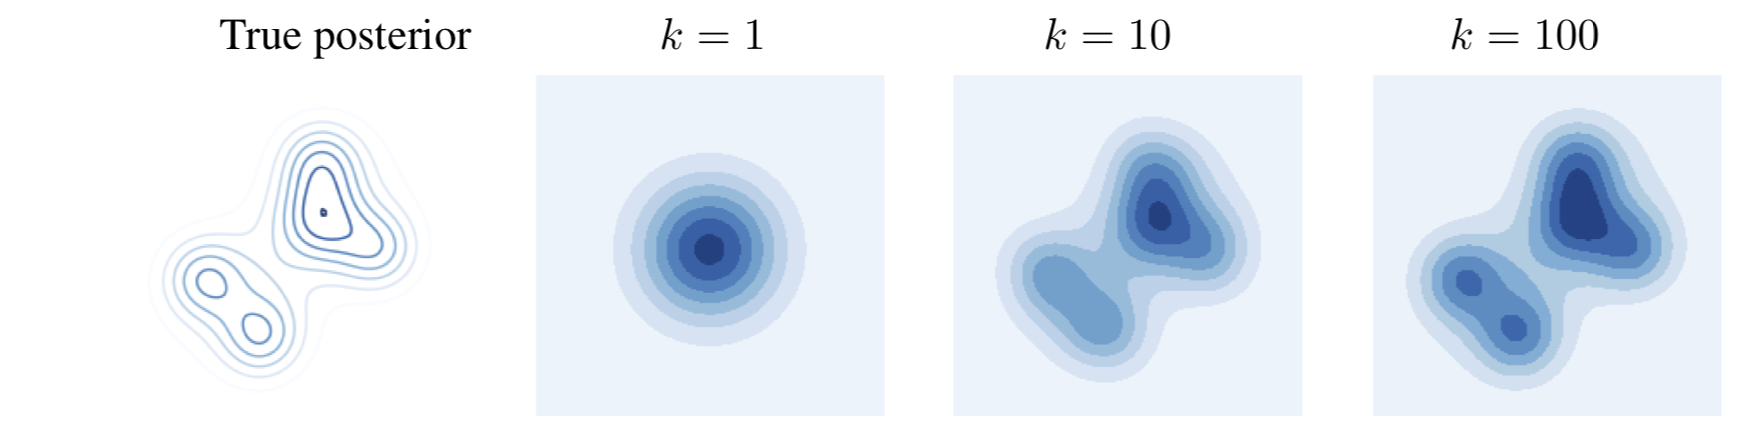
\includegraphics[width=\linewidth]{figs/IWAE_1.png}
		\end{figure}
	\end{block}

	\myfootnotewithlink{https://arxiv.org/abs/1704.02916}{Cremer C., Morris Q., Duvenaud D. Reinterpreting Importance-Weighted Autoencoders, 2017}
\end{frame}
%=======
\begin{frame}{IWAE}
	\begin{block}{Objective}
		\vspace{-0.5cm}
		\[
		\mathcal{L}_K (q, \btheta)  = \mathbb{E}_{\bz_1, \dots, \bz_K \sim q(\bz | \bx, \bphi)} \log \left( \frac{1}{K}\sum_{k=1}^K\frac{p(\bx, \bz_k | \btheta)}{q(\bz_k| \bx, \bphi)} \right) \rightarrow \max_{\bphi, \btheta}.
		\]
		\vspace{-0.3cm}
	\end{block}
	\begin{block}{Gradient}
		\vspace{-0.3cm}
		\[
		\Delta_K = \nabla_{\btheta, \bphi} \log \left( \frac{1}{K}\sum_{k=1}^K\frac{p(\bx, \bz_k | \btheta)}{q(\bz_k| \bx, \bphi)} \right), \quad \bz_k \sim q(\bz | \bx, \bphi).
		\]
		\vspace{-0.3cm}
	\end{block}
	\begin{block}{Theorem}
		\vspace{-0.4cm}
		\[
			\text{SNR}_K = \frac{\bbE [\Delta_K]}{\sigma(\Delta_K)}; \quad
			\text{SNR}_K(\btheta) = O(\sqrt{K}); \quad 
			\text{SNR}_K(\bphi) = O\left(\sqrt{\frac{1}{K}}\right).
		\]
		Hence, increasing $K$ vanishes gradient signal of inference network $q(\bz | \bx, \bphi)$.
	\end{block}

	\myfootnotewithlink{https://arxiv.org/abs/1802.04537}{Rainforth T. et al. Tighter variational bounds are not necessarily better, 2018}
\end{frame}
%=======
\begin{frame}{IWAE}
	\begin{block}{Theorem}
		\vspace{-0.5cm}
		\[
			\text{SNR}_K = \frac{\bbE [\Delta_K]}{\sigma(\Delta_K)}; \quad
			\text{SNR}_K(\btheta) = O(\sqrt{K}); \quad 
			\text{SNR}_K(\bphi) = O\left(\sqrt{\frac{1}{K}}\right).
		\]
		\vspace{-0.8cm}
	\end{block}
		\begin{minipage}[t]{0.5\columnwidth}
			\begin{figure}[h]
				\centering
				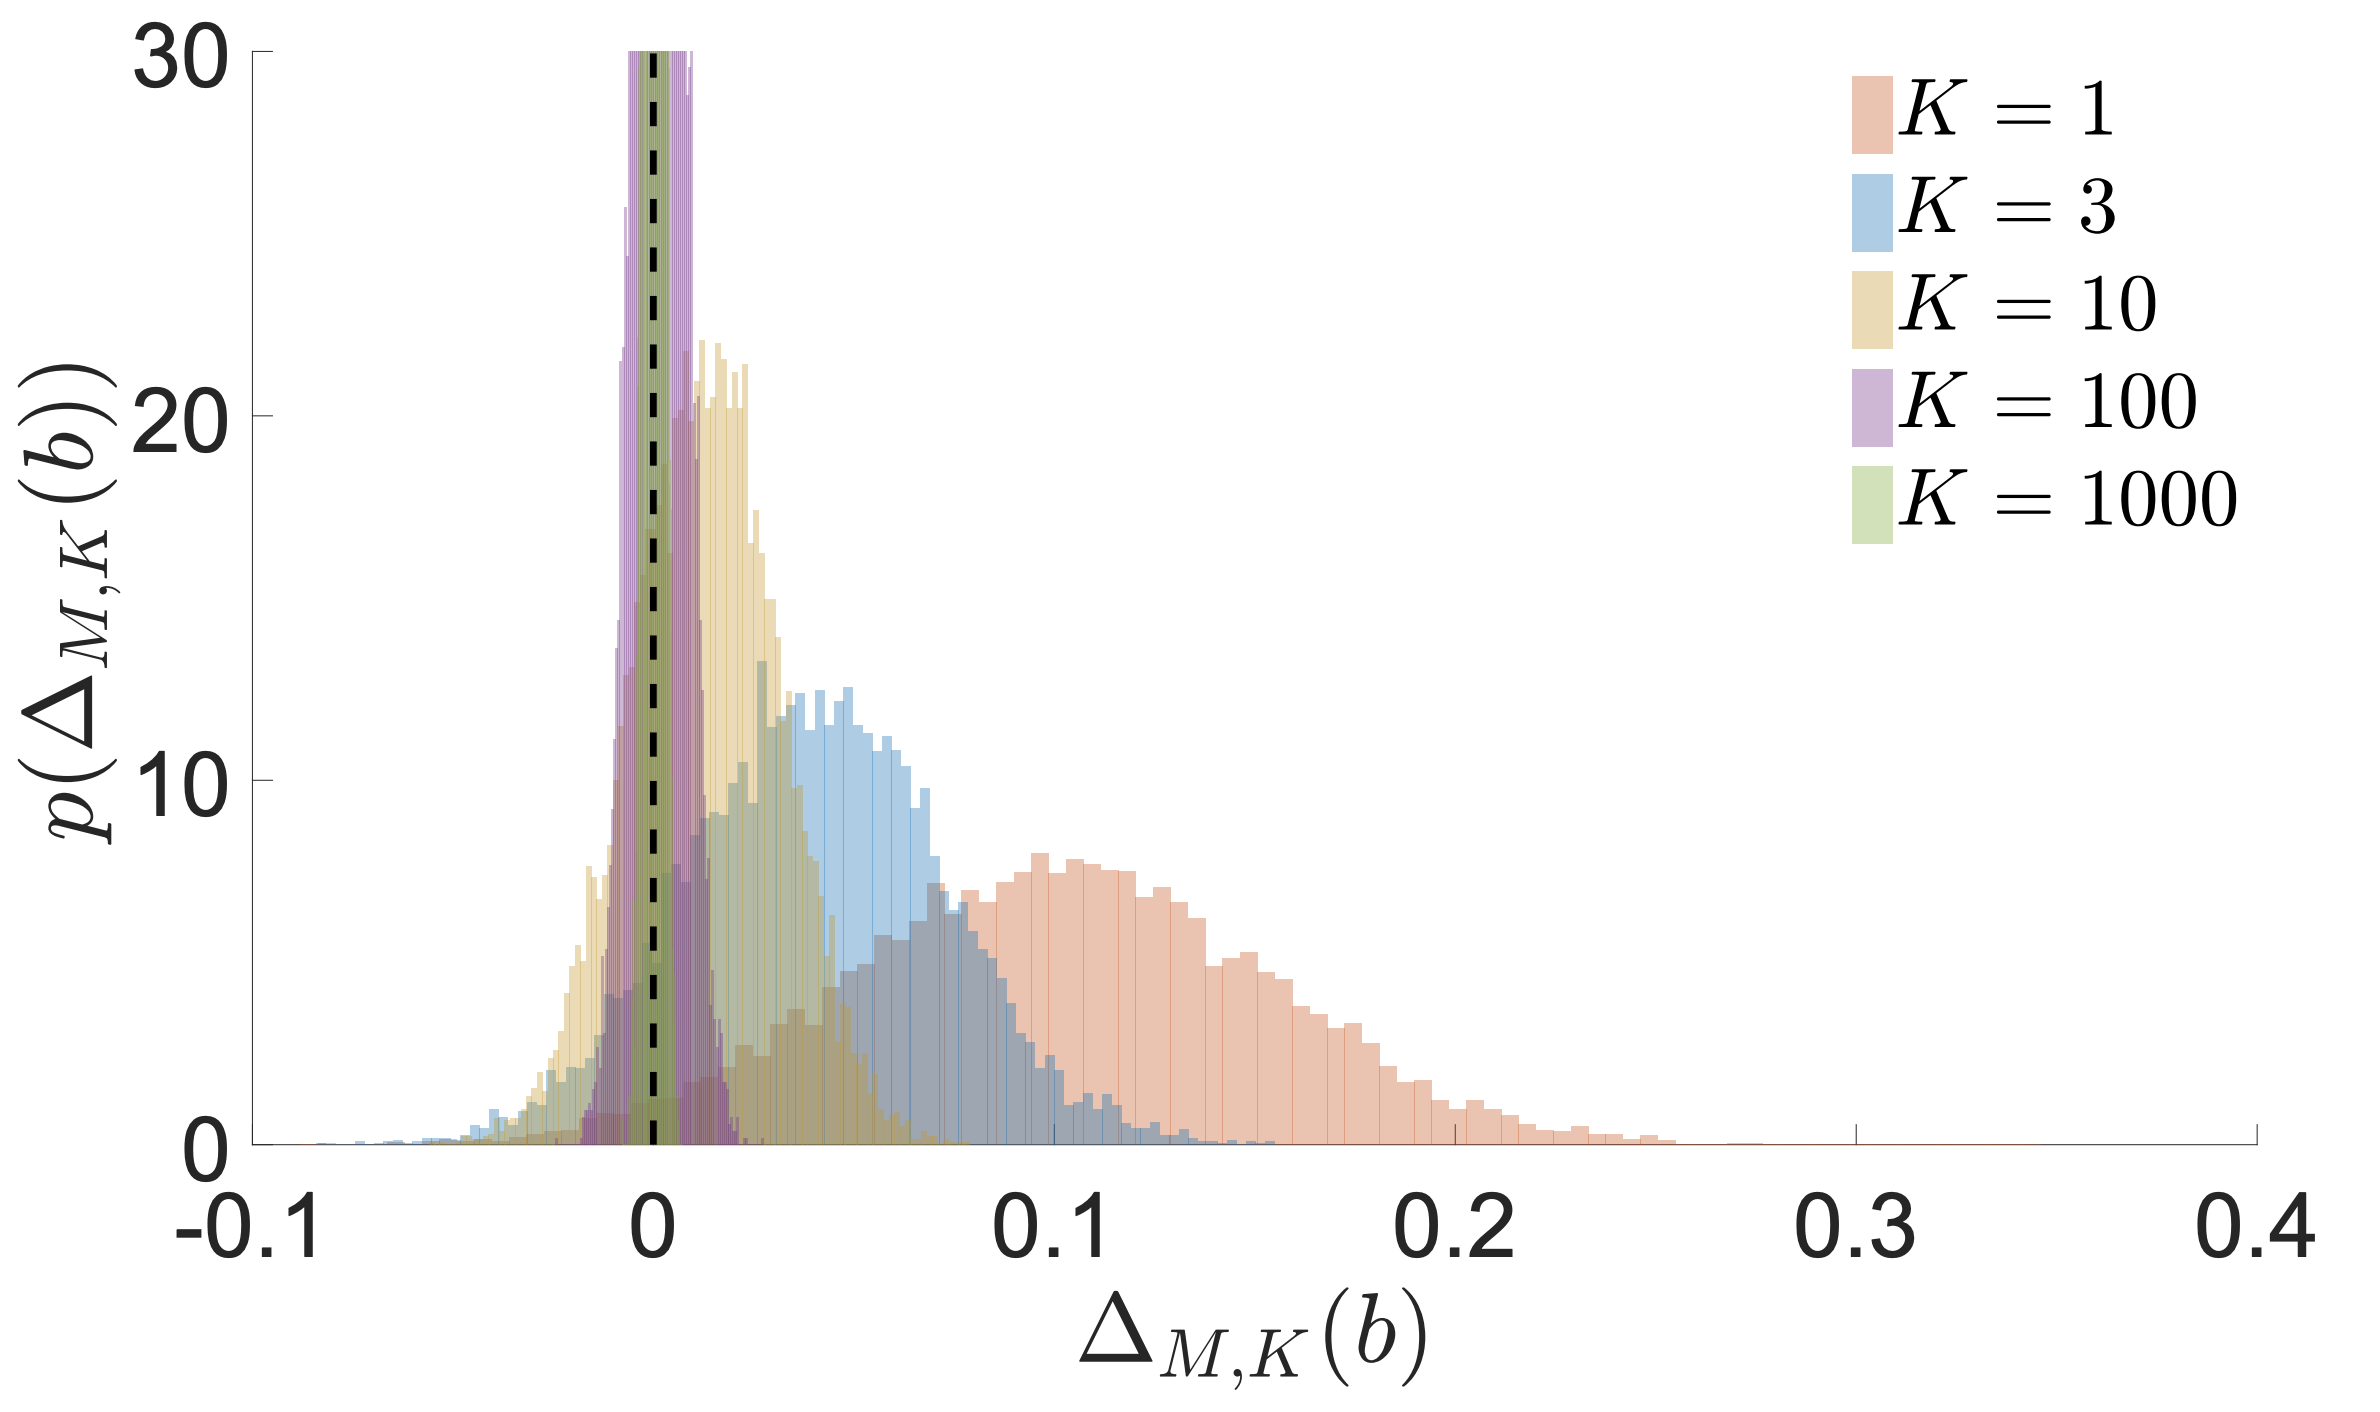
\includegraphics[width=1.\linewidth]{figs/IWAE_SNR_1.png}
			\end{figure}
		\end{minipage}%
		\begin{minipage}[t]{0.5\columnwidth}
			\begin{figure}[h]
				\centering
				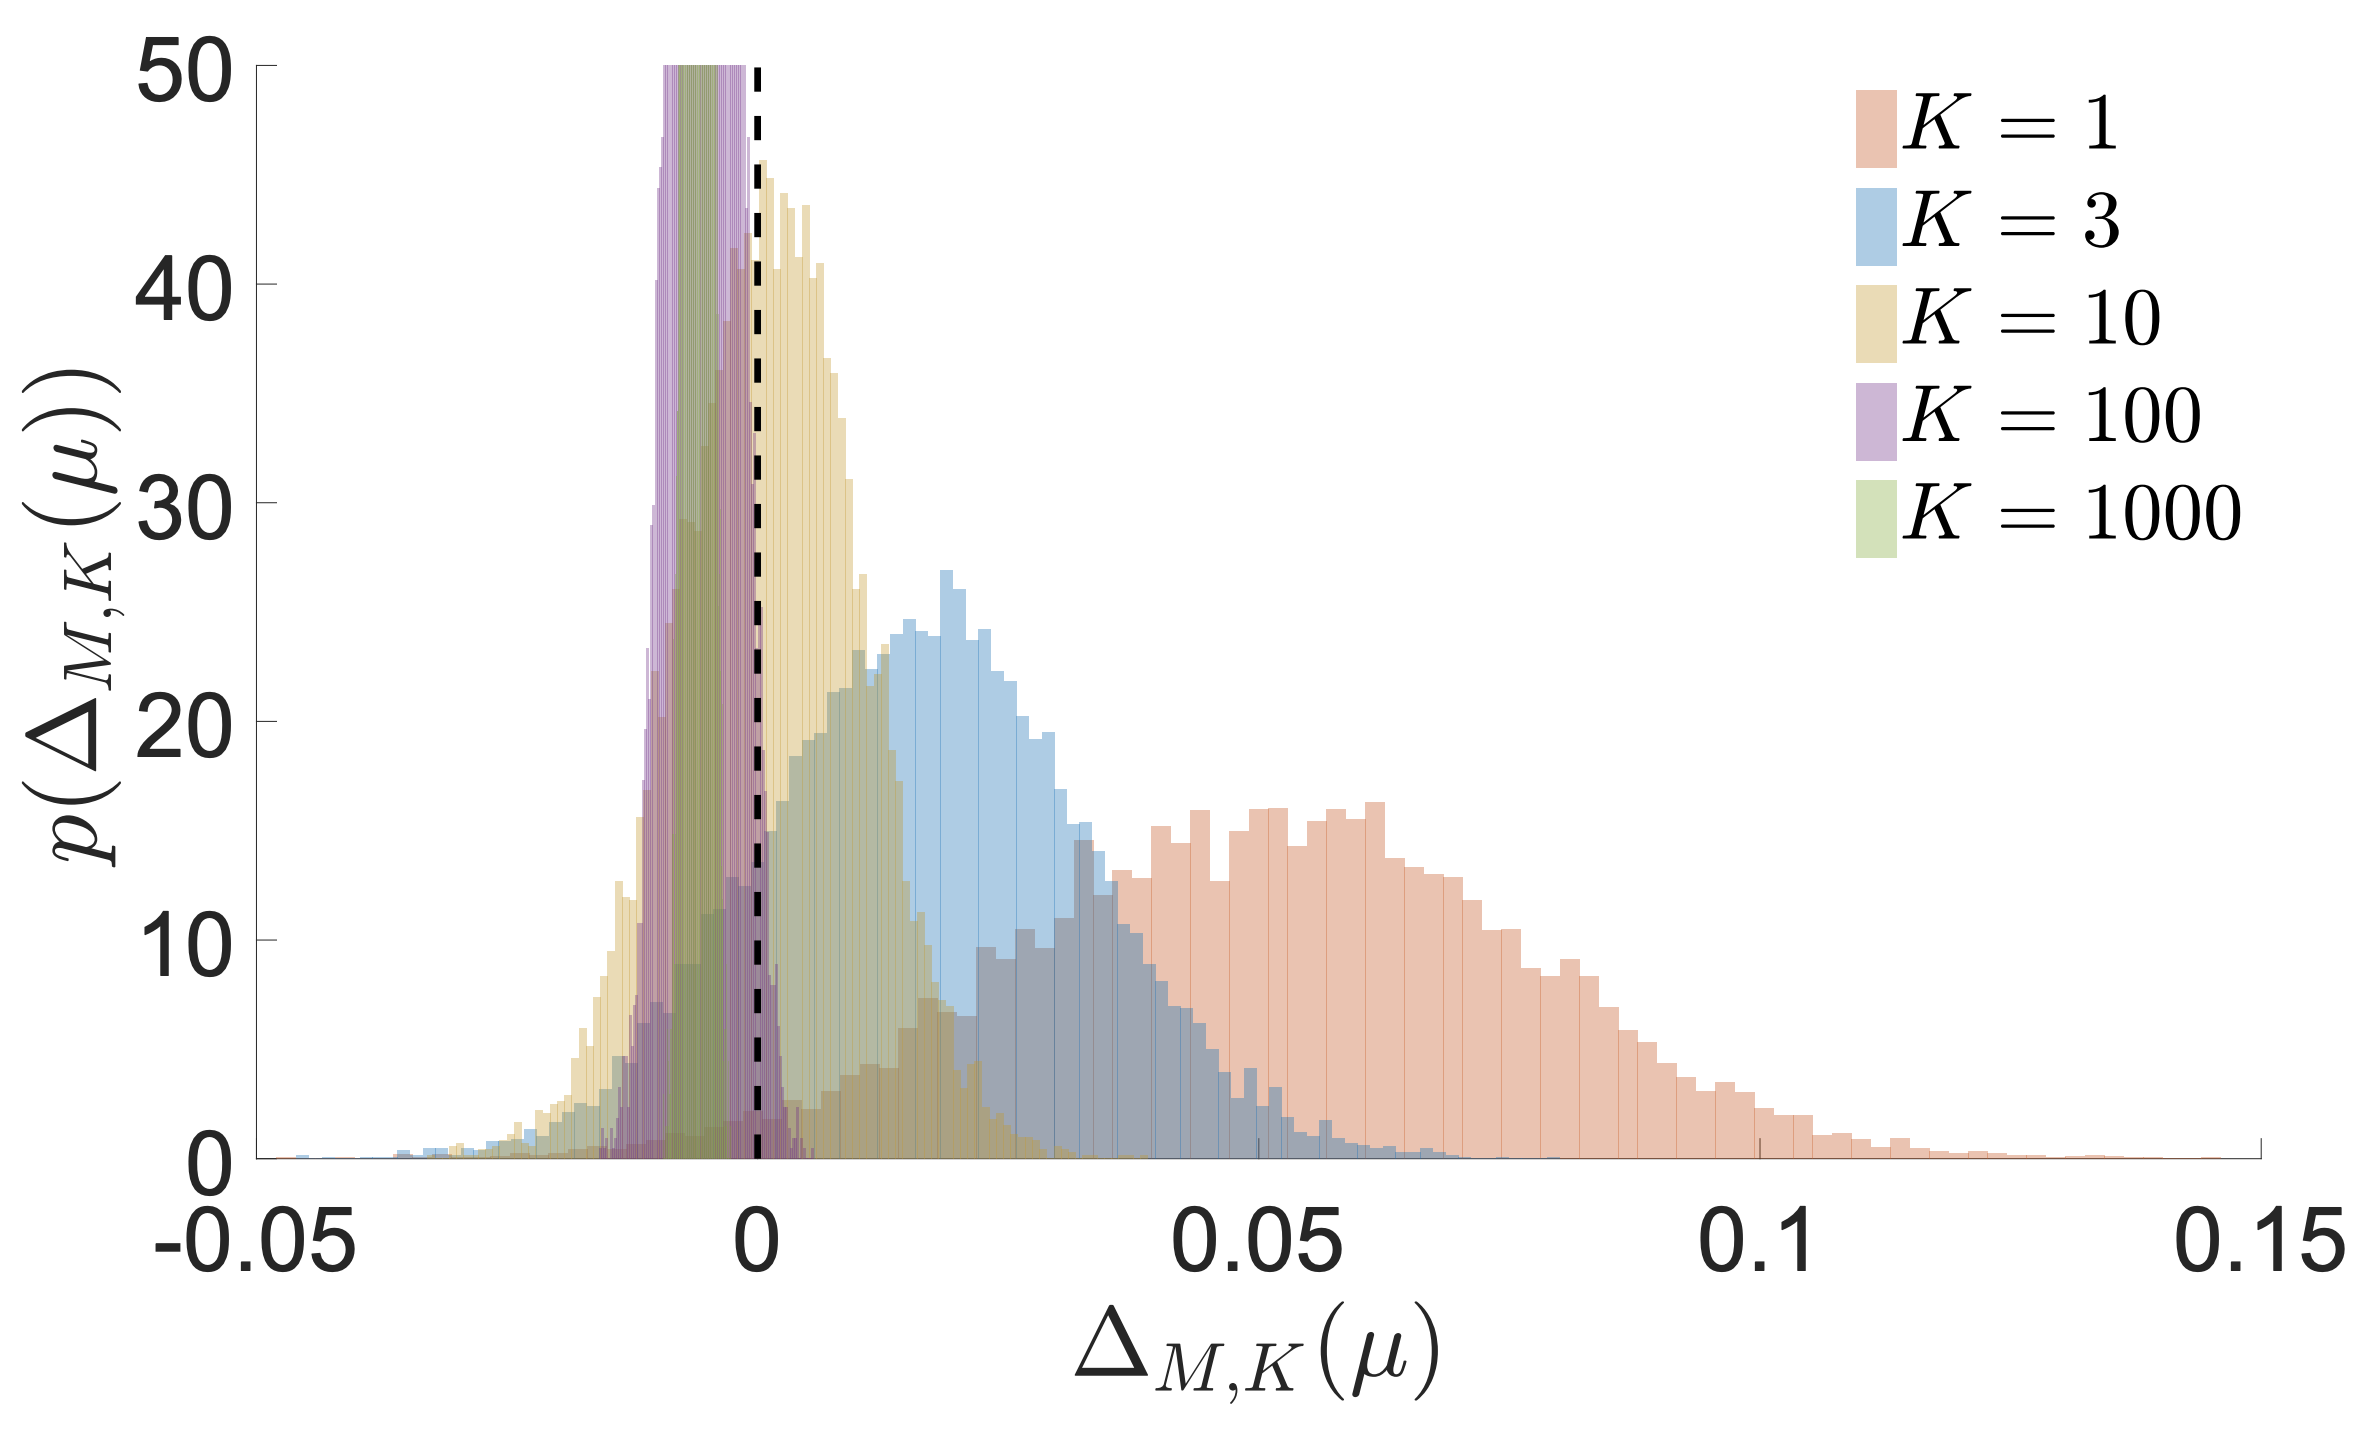
\includegraphics[width=1.\linewidth]{figs/IWAE_SNR_2.png}
			\end{figure}
		\end{minipage}
	\begin{itemize}
		\item IWAE makes the variational bound tighter and extends the class of variational distributions.
		\item Gradient signal becomes really small, training is complicated.
		\item IWAE is very popular technique as a quality measure for VAE models.
	\end{itemize}
	\myfootnotewithlink{https://arxiv.org/abs/1802.04537}{Rainforth T. et al. Tighter variational bounds are not necessarily better, 2018}
\end{frame}
%=======
\begin{frame}{Summary}
	\begin{itemize}
		\item Linear flows try to parametrize set of invertible matrices via matrix decompositions.
		\vfill
		\item More powerful decoder in VAE leads to more expressive generative model. However, too expressive decoder could lead to the posterior collapse.
		\vfill
		\item The decoder weakening is a set of techniques to avoid the posterior collapse.
		\vfill
		\item The IWAE could get the tighter lower bound to the likelihood, but the training of such model becomes more difficult.
	\end{itemize}
\end{frame}
%=======
\end{document} 